{\color{bleu}\chapter{Conception de la Solution }}
\thispagestyle{empty}
\newpage

% ============================================================
{\color{bleu} \section{Introduction}}
% ============================================================

\par Ce chapitre présente la conception détaillée de l'infrastructure Cloud privée hyperconvergée que nous proposons. Sur la base des technologies retenues dans le chapitre précédent, Proxmox VE, Ceph et Open vSwitch, nous décrivons ici les choix architecturaux guidant la construction de chaque couche de l'infrastructure : physique, réseau, stockage et applicative. Nous présentons également la conception du mécanisme d'équilibrage dynamique de charge CLBS que nous développons en complément de la stack de base, ainsi que les outils d'automatisation retenus pour le déploiement et le provisionnement.\\

\par L'objectif de ce chapitre est de fournir une vision complète et cohérente de l'architecture avant toute phase d'implémentation, en justifiant chaque décision de conception par des contraintes techniques, des recommandations officielles ou des exigences fonctionnelles identifiées dans le chapitre précédent.\\

% ============================================================
{\color{bleu} \section{Vue Globale de l'Architecture Proposée}}
% ============================================================

\par L'architecture proposée repose sur un modèle à trois couches superposées et interdépendantes, chacune apportant une dimension essentielle à l'infrastructure hyperconvergée.\\

\par La première couche est la \textbf{couche physique}, constituée de trois serveurs Dell PowerEdge R720 mis à disposition par le Centre d'innovation de Sonatrach. Proxmox VE sera installé directement en mode bare metal sur chacun de ces serveurs, sans aucune couche de virtualisation intermédiaire. Cette approche garantit des performances maximales et simplifie considérablement le modèle de dépannage.\\

\par La deuxième couche est la \textbf{couche de virtualisation et de cluster}, composée des trois n\oe{}uds Proxmox physiques (PVE-01, PVE-02, PVE-03) interconnectés via le réseau de Sonatrach. Ces trois n\oe{}uds formeront un cluster Proxmox haute disponibilité géré par Corosync pour le consensus et la détection des pannes. Chaque n\oe{}ud exécutera simultanément les daemons Ceph nécessaires au stockage distribué et une instance Open vSwitch pour la gestion du trafic réseau, avec des tunnels VxLAN pour la segmentation logique. Cette convergence des rôles au sein de chaque n\oe{}ud est l'expression directe du principe HCI.\\

\par La troisième couche est la \textbf{couche applicative et de services}, hébergée par le cluster Proxmox. Elle comprendra une VM OPNsense assurant le routage inter-réseaux, le filtrage par pare-feu et les services DHCP internes, les VMs de démonstration constituant l'application Sona-Web, ainsi que les services d'infrastructure transversaux : le mécanisme CLBS que nous développons, la stack de monitoring (InfluxDB, Prometheus et Grafana), et les outils d'automatisation Ansible.\\

\par Ces trois couches interagiront de manière unifiée depuis l'interface d'administration centralisée Proxmox, accessible sur le réseau de management 192.168.10.0/24 déjà en place dans l'infrastructure Sonatrach. La figure 3-1 illustre cette organisation globale.\\

\begin{figure}[H]
    \begin{center}
        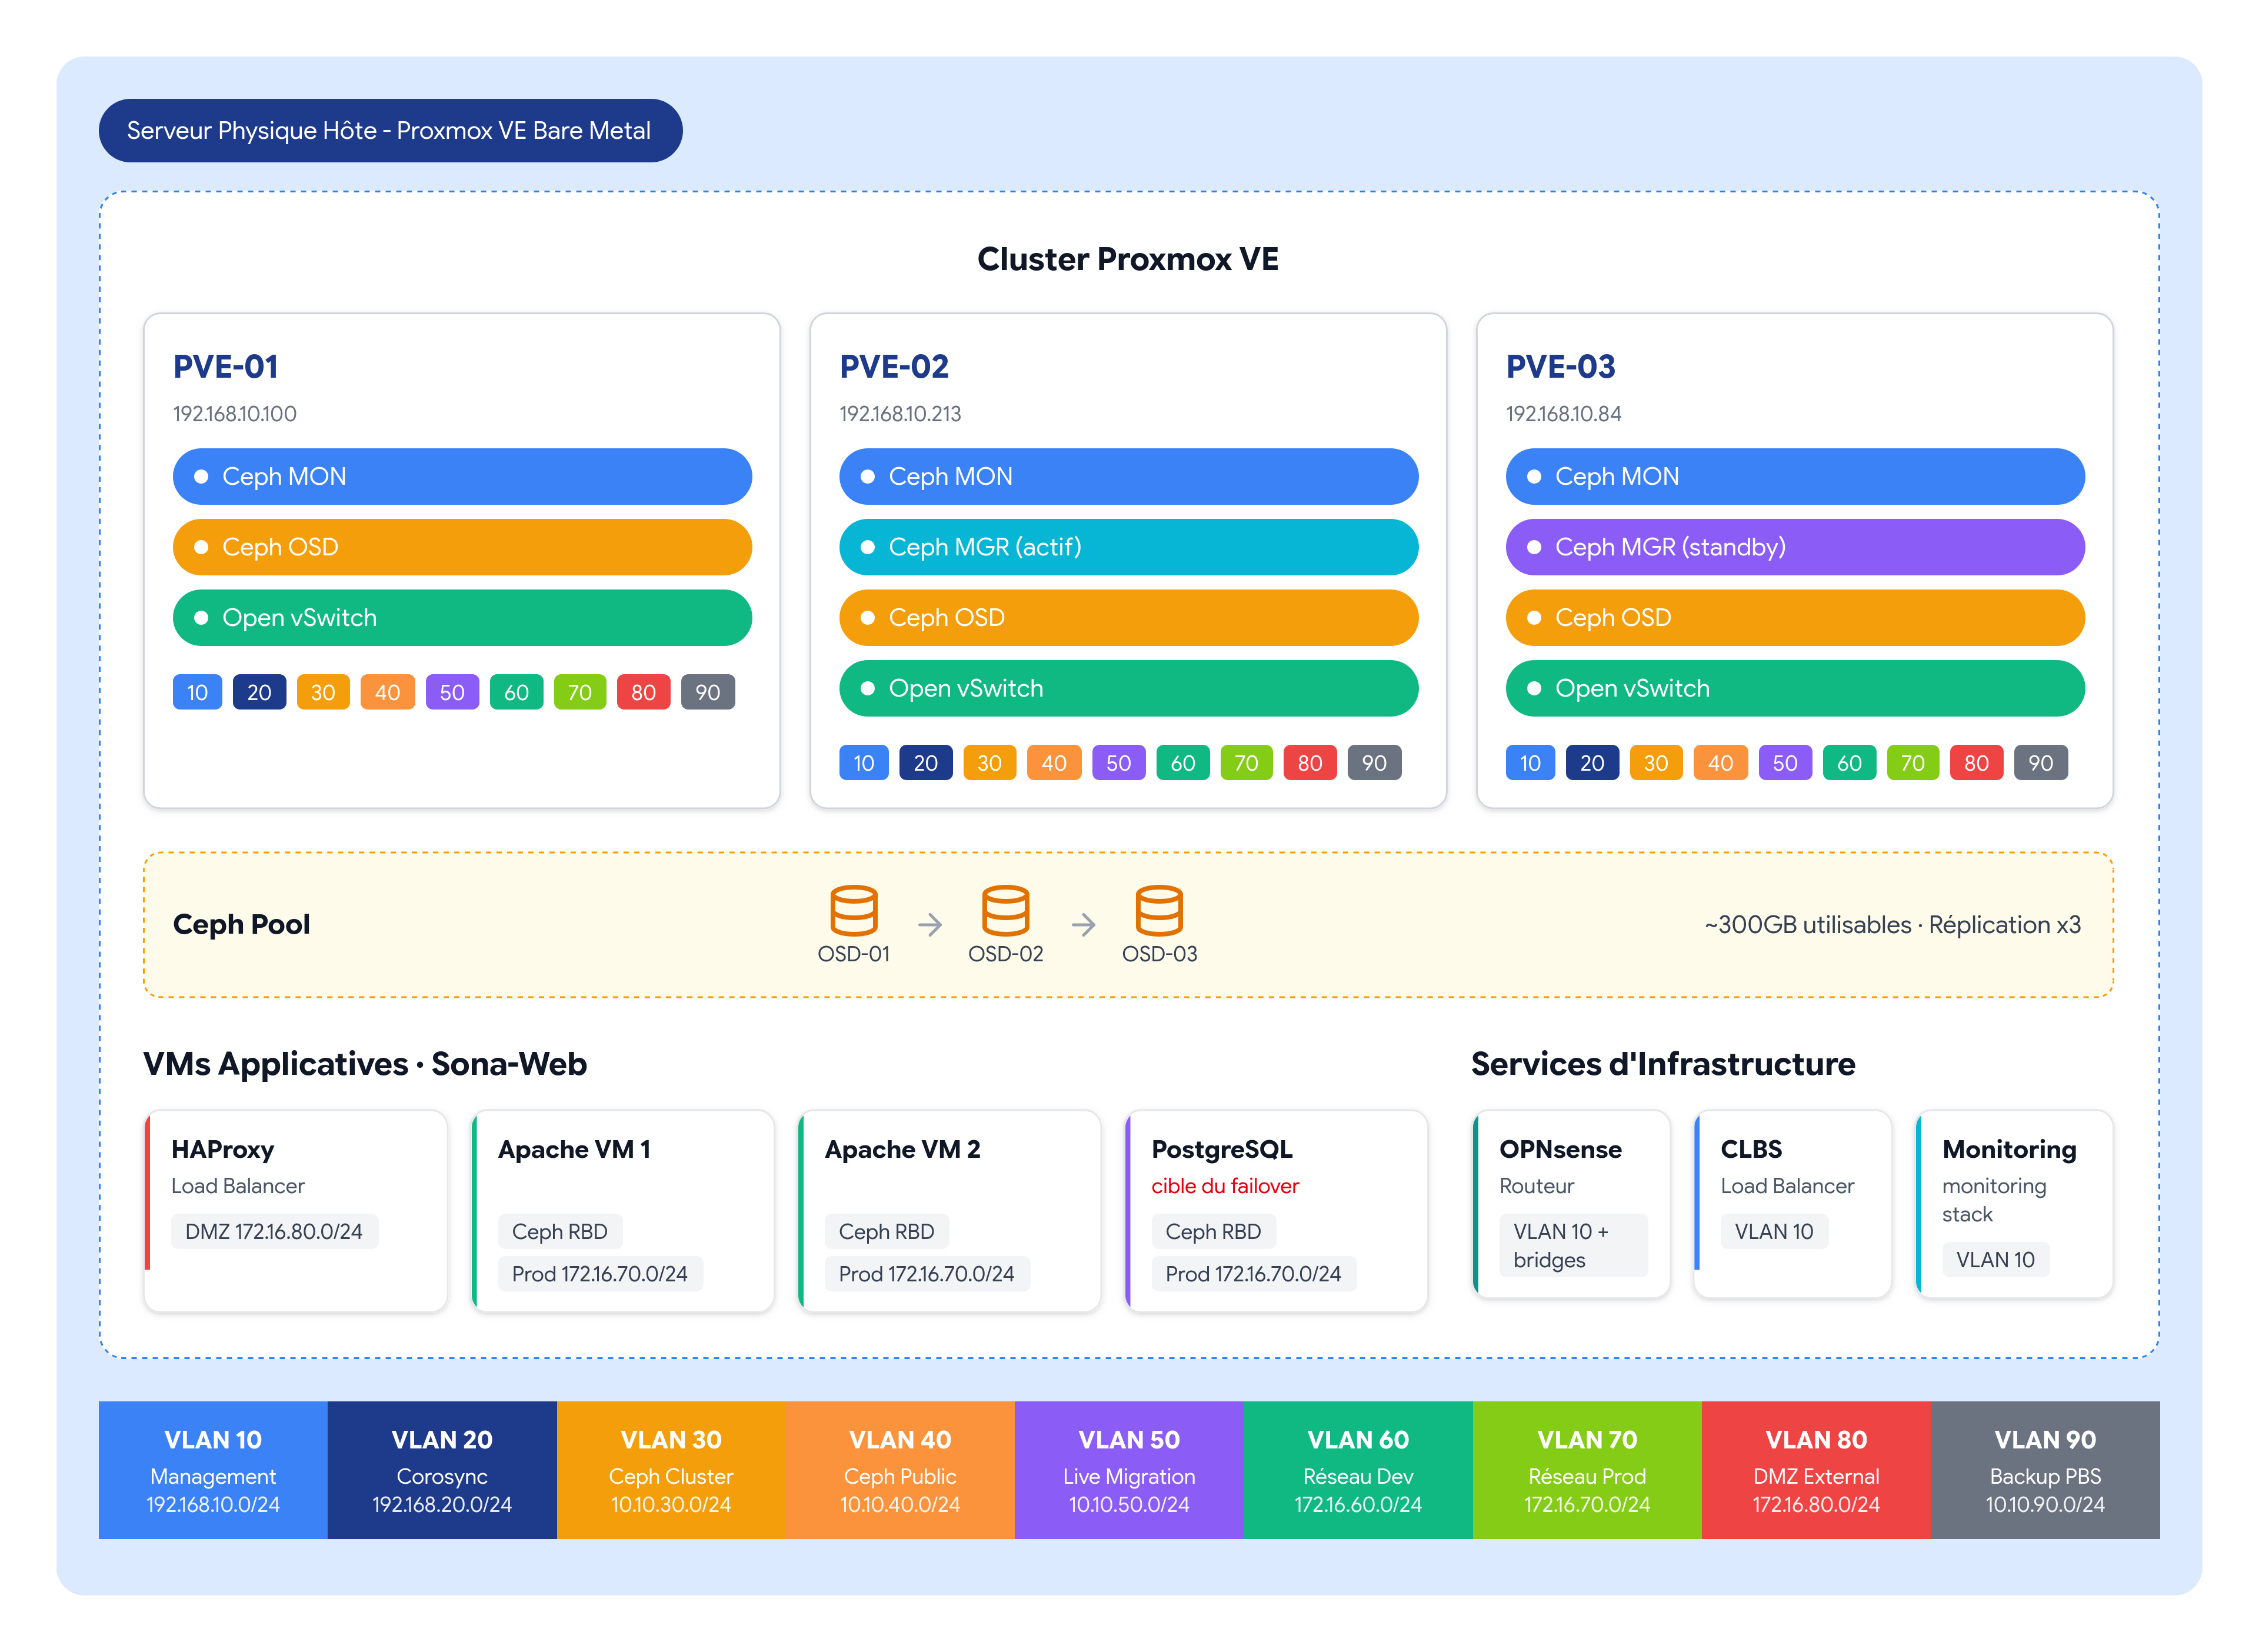
\includegraphics[width=0.9\textwidth]{image/ch3/architecture-hci.jpg}
        \caption{Architecture Globale de l'Infrastructure}
        \label{fig:arch-globale}
    \end{center}
\end{figure}


% %%%%%%%%%%%%%%%%%%%%%%%%%%%%%%%%%%%%%%%%%%%%%%%%%%%%%%%%%%%%
% PARTIE 1 : COMPUTE
% %%%%%%%%%%%%%%%%%%%%%%%%%%%%%%%%%%%%%%%%%%%%%%%%%%%%%%%%%%%%

{\color{bleu} \section{Partie I : Compute}}

% ============================================================
{\color{bleu} \section{Architecture Physique}}
% ============================================================

{\color{bleuu} \subsection{Infrastructure Physique}}

\par L'infrastructure physique est constituée de trois serveurs Dell PowerEdge R720 mis à disposition par le Centre d'innovation de Sonatrach. Ces serveurs constitueront les trois n\oe{}uds physiques du cluster Proxmox : PVE-01, PVE-02 et PVE-03. Proxmox VE sera installé directement en mode bare metal sur chacun d'eux, sans couche de virtualisation intermédiaire.\\

\par Le Dell PowerEdge R720 est un serveur rack 2U de la gamme Enterprise de Dell, reconnu pour sa robustesse et sa capacité d'extension. Il est équipé de processeurs Intel Xeon E5-2600 et supporte jusqu'à 768 GB de RAM, ce qui en fait une plateforme adaptée aux charges de virtualisation intensive et au stockage distribué. Dans notre déploiement, chaque serveur sera configuré avec 64 GB de RAM et deux disques SAS répartis selon les rôles définis ci-dessous.\\

\par \textbf{Allocation des disques par n\oe{}ud}\\

\par Chaque serveur disposera de deux disques SAS répartis en deux catégories fonctionnelles, conformément aux recommandations Proxmox et Ceph concernant la séparation des I/O système et stockage :\\

\begin{itemize}
    \item \textbf{Disque système (sda -- 1 x 300 GB SAS) :} dédié au système d'exploitation Proxmox VE. Cette séparation garantit que les opérations de réplication Ceph ne concurrencent pas les I/O système du n\oe{}ud, conformément aux recommandations officielles Proxmox [10].
    \item \textbf{Disque OSD Ceph (sdb -- 1 x 300 GB SAS) :} affecté à un OSD Ceph distinct, contribuant au stockage distribué du cluster. Chaque n\oe{}ud apportera ainsi 1 OSD au pool global.
\end{itemize}

\begin{center}
\begin{tabular}{|p{3cm}|p{3cm}|p{3cm}|p{4cm}|}
\hline
\textbf{Composant} & \textbf{Valeur par n\oe{}ud} & \textbf{Total cluster} & \textbf{Justification} \\
\hline
\textbf{Modèle serveur} & Dell PowerEdge R720 & 3 serveurs & Fourni par Sonatrach \\
\hline
\textbf{RAM} & 64 GB & 192 GB & Proxmox + Ceph + VMs [10][14] \\
\hline
\textbf{Disque OS (sda)} & 1 x 300 GB SAS & 3 x 300 GB & Isolation I/O hôte / Ceph [10] \\
\hline
\textbf{Disque OSD (sdb)} & 1 x 300 GB SAS & 3 x 300 GB & 1 OSD par n\oe{}ud [12][13] \\
\hline
\textbf{IP Management} & Voir tableau 3-4 & & VxLAN 10 -- réseau Sonatrach \\
\hline
\end{tabular}
\end{center}
\noindent \textit{Tableau 3-1 : Dimensionnement physique des serveurs Dell PowerEdge R720}\\

% ============================================================
{\color{bleu} \section{Architecture du Cluster Proxmox}}
% ============================================================

{\color{bleuu} \subsection{Organisation du Cluster}}

\par Le cluster Proxmox sera constitué de trois n\oe{}uds physiques identiques interconnectés via le réseau de Sonatrach. Chaque n\oe{}ud exécutera Proxmox VE en bare metal sur un serveur Dell PowerEdge R720 dédié. Le trafic Corosync sera transporté sur un réseau logique dédié (VxLAN ID 20) afin de garantir la stabilité du quorum indépendamment des autres flux réseau.\\

\par Cette organisation à trois n\oe{}uds physiques est le minimum requis par Proxmox pour garantir un quorum stable et éviter les situations de split-brain [21]. La défaillance complète d'un n\oe{}ud physique sera absorbée par le mécanisme HA de Proxmox, les deux n\oe{}uds survivants maintenant le quorum (2/3) et continuant à opérer normalement.\\

\begin{center}
\begin{tabular}{|p{4cm}|p{4cm}|p{5cm}|}
\hline
\textbf{N\oe{}ud} & \textbf{Nom d'hôte} & \textbf{Adresse IP Management (192.168.10.0/24)} \\
\hline
N\oe{}ud 1 & PVE-01 & 192.168.10.100 \\
\hline
N\oe{}ud 2 & PVE-02 & 192.168.10.213 \\
\hline
N\oe{}ud 3 & PVE-03 & 192.168.10.84 \\
\hline
\end{tabular}
\end{center}
\noindent \textit{Tableau 3-2 : Adresses IP de management des n\oe{}uds Proxmox physiques}\\

{\color{bleuu} \subsection{Mécanisme de Quorum et Corosync}}

\par Corosync est le framework de communication de cluster utilisé par Proxmox pour assurer le consensus entre les n\oe{}uds. Il enverra des messages de heartbeat entre les n\oe{}uds à intervalles réguliers via le réseau logique VxLAN ID 20 dédié. Lorsqu'un n\oe{}ud cessera de répondre, Corosync déclenchera une procédure de vote pour déterminer si le cluster dispose encore du quorum nécessaire pour continuer à opérer [20].\\

\par Le quorum dans un cluster de trois n\oe{}uds est atteint dès que deux n\oe{}uds sur trois sont opérationnels. La perte de deux n\oe{}uds simultanément entraînerait la perte du quorum et le gel du cluster pour éviter toute corruption des données, comportement conforme aux recommandations de sécurité Proxmox [6].\\

{\color{bleuu} \subsection{Haute Disponibilité}}

\par Le mécanisme de haute disponibilité (HA) de Proxmox s'appuiera sur Corosync pour la détection des pannes et sur le Resource Manager HA pour les décisions de basculement [6]. Lorsqu'un n\oe{}ud sera déclaré défaillant, le HA Manager identifiera les VMs qui y résidaient et déclenchera leur redémarrage automatique sur un des n\oe{}uds survivants.\\

\par Ce mécanisme est rendu possible par le stockage partagé Ceph : les disques des VMs étant stockés sur le pool Ceph commun et accessibles depuis n'importe quel n\oe{}ud du cluster, le redémarrage d'une VM sur un n\oe{}ud différent ne nécessitera aucun transfert de données. La VM redémarrera directement depuis le volume Ceph RBD existant, ce qui minimise le temps de récupération après panne (RTO). Selon la documentation Proxmox, ce délai de basculement est typiquement compris entre 60 et 120 secondes.\\

\par Dans notre architecture, toutes les VMs de l'application Sona-Web seront configurées en mode HA, avec une priorité de basculement définie pour garantir que le load balancer HAProxy est redémarré en premier, suivi des serveurs web, puis de la base de données PostgreSQL.\\

{\color{bleuu} \subsection{Matrice des Scénarios de Défaillance}}

\par Le tableau suivant recense les scénarios de défaillance envisagés 
et le comportement attendu du système dans chacun d'eux :\\

\begin{center}
\begin{tabular}{|p{2.8cm}|p{2.5cm}|p{7cm}|p{2cm}|}
\hline
\textbf{Scénario} & \textbf{Composant affecté} & \textbf{Comportement du système} & \textbf{RTO estimé} \\
\hline
Panne d'un n\oe{}ud physique & PVE-01, PVE-02 ou PVE-03 &
Corosync détecte la perte de heartbeat. Le HA Manager redémarre les
VMs HA sur les n\oe{}uds survivants (quorum 2/3 maintenu). Ceph passe
en état \texttt{degraded} mais reste accessible (\texttt{min\_size=2}).
& 60--120 s \\
\hline
Panne d'un OSD Ceph & Disque \texttt{sdb} sur un n\oe{}ud &
Ceph marque l'OSD \texttt{down} puis \texttt{out}. Le pool passe en
état \texttt{degraded} (2 répliques sur 3) mais les I/O continuent.
Dès rétablissement, un \textit{backfill} automatique reconstitue la
troisième réplique.
& Aucune coupure \\
\hline
Panne du MGR actif & PVE-02 (MGR actif) &
Le MGR en standby (PVE-03) prend le relais automatiquement.
L'endpoint Prometheus (port 9283) reste disponible sans intervention
manuelle.
& \textless{} 30 s \\
\hline
Panne de deux n\oe{}uds simultanés & Deux des trois n\oe{}uds &
Perte du quorum Corosync et Ceph. Le n\oe{}ud survivant se gèle pour
prévenir tout split-brain. Le cluster devient inaccessible et une
intervention manuelle est requise.
& N/A \\
\hline
Panne de la VM OPNsense & VM routeur/pare-feu &
Proxmox HA redémarre la VM sur un n\oe{}ud survivant. Le trafic
inter-réseaux est interrompu pendant la durée du redémarrage, ce qui
constitue la limite connue de cette approche par rapport à un
basculement CARP sans interruption.
& 60--120 s \\
\hline
Partition réseau (split-brain) & Réseau VxLAN 20 (Corosync) &
Le groupe minoritaire (1 n\oe{}ud) perd le quorum et se gèle. Le
groupe majoritaire (2 n\oe{}uds) continue d'opérer. Le gel prévient
toute écriture divergente sur Ceph.
& Aucune coupure côté majoritaire \\
\hline
Défaillance du service CLBS & VM CLBS &
Aucun impact applicatif. Le service redémarre automatiquement
(\texttt{Restart=always} dans l'unit systemd). Si la VM elle-même
est défaillante, Proxmox HA la redémarre sur un autre n\oe{}ud.
& Aucune coupure applicative \\
\hline
\end{tabular}
\end{center}
\noindent \textit{Tableau 3-X : Matrice des scénarios de défaillance et comportements attendus}\\ee

% ============================================================
{\color{bleu} \section{Mécanisme d'Équilibrage Dynamique : CLBS}}
% ============================================================

{\color{bleuu} \subsection{Contexte et Besoin}}

\par Proxmox VE intègre nativement un mécanisme de haute disponibilité réactif : lorsqu'un n\oe{}ud tombe en panne, les VMs qui y résidaient sont automatiquement redémarrées sur les n\oe{}uds survivants. Cependant, Proxmox ne dispose d'aucun mécanisme proactif d'équilibrage de charge, contrairement à VMware vSphere qui propose le DRS (Distributed Resource Scheduler) [18].\\

\par Sans équilibrage proactif, un cluster Proxmox peut se retrouver dans une situation où un n\oe{}ud est saturé à 90\% de CPU tandis qu'un autre n\oe{}ud reste à 20\% d'utilisation. Proxmox n'intervient pas dans ce cas, laissant le déséquilibre persister et dégradant les performances des VMs sur le n\oe{}ud surchargé. Ce déséquilibre représente un gaspillage significatif de ressources et une dégradation de la qualité de service [18].\\

{\color{bleuu} \subsection{Base Algorithmique : CSLB}}

\par Notre mécanisme, que nous nommons \textbf{CLBS (Central Load Balancing Scheduler)}, est une adaptation du CSLB (Central Scheduler Load Balancing) [17]. L'algorithme CSLB original repose sur cinq phases : évaluation de charge, détermination de rentabilité, calcul du vecteur de transfert, sélection de VM et exécution de la migration.\\

\par Dans CSLB, la charge CPU de chaque n\oe{}ud est évaluée par rapport à un seuil dynamique (moyenne des charges de tous les n\oe{}uds). Une bande modérée est calculée autour de ce seuil selon la formule :

\begin{center}
$\text{seuil} = \frac{\sum_{i=1}^{n} \alpha_i}{n}$, \quad
$\text{diff} = |\text{seuil} - \frac{\alpha_{min} + \alpha_{max}}{2}|$ \\
$\alpha_i $: le CPU du nœud i \\
$n :$ Nombre du nœuds
\end{center}

\par La bande modérée est définie à $\pm \max(\text{diff}, 10\%)$ autour du seuil. Les n\oe{}uds hors bande modérée sont candidats à une action d'équilibrage.\\

{\color{bleuu} \subsection{Modifications Apportées au CSLB}}

\par Notre adaptation du CSLB intègre plusieurs modifications
significatives par rapport à l'algorithme original. Le service est
implémenté en \textbf{Go} (Golang), retenu pour sa faible empreinte
mémoire, sa gestion native de la concurrence via les goroutines, et
la simplicité de son déploiement sous forme de binaire statique dans
un service systemd.\\

\par \textbf{Extension à la RAM.} Le CSLB original ne considère que
le CPU. Notre implémentation étend l'évaluation à la RAM, calculant
une bande modérée indépendante pour chaque métrique. Un n\oe{}ud est
considéré surchargé si l'une ou l'autre dépasse sa bande respective.\\

\par \textbf{Seuil minimum de migration.} Une migration n'est
déclenchée que si la charge du n\oe{}ud surchargé dépasse un seuil
absolu de 50\% (CPU ou RAM). En dessous, même si le n\oe{}ud est
statistiquement hors de sa bande, la migration est jugée non rentable,
évitant des déplacements inutiles dans un cluster globalement
sous-chargé.\\

\par \textbf{Sélection du n\oe{}ud destination pondérée avec
vérification préalable.} Le choix du n\oe{}ud destination se fonde
sur un score de différentiel pondéré :

\begin{center}
$\text{score} = \Delta_{CPU} \times 0.7 + \Delta_{RAM} \times 0.3$
\end{center}

\par Avant de valider la destination, CLBS simule l'état post-migration
du n\oe{}ud cible en y ajoutant la consommation de la VM candidate.
Si le résultat dépasse la bande haute, ce n\oe{}ud est écarté et le
candidat suivant est évalué, évitant de transférer la surcharge d'un
n\oe{}ud à l'autre.\\

\par \textbf{Exclusion des VMs système.} OPNsense, la VM de monitoring
et la VM CLBS elle-même sont explicitement exclues du périmètre de
migration : migrer l'une d'elles interromprait respectivement le
routage inter-réseaux, les métriques nécessaires aux décisions CLBS,
ou le service lui-même.\\

\par \textbf{Cadence et unicité de migration par cycle.} CLBS
s'exécute toutes les 60 secondes et ne peut déclencher qu'une seule
migration par cycle. Cette contrainte laisse au cluster le temps
d'intégrer le changement de charge, prévient les effets de cascade,
et exclut explicitement la VM migrée du cycle suivant.\\

\par \textbf{Cooldown post-migration.} Après chaque migration réussie,
une période de repos de \textbf{5 minutes} est appliquée, garantissant
que les métriques InfluxDB, lissées sur une fenêtre glissante de
5 minutes, ont intégré l'impact de la migration avant toute nouvelle
décision.\\

\par \textbf{Mécanisme anti-oscillation et disjoncteurs.} Plusieurs
niveaux de protection contre les comportements instables sont mis
en place :

\begin{itemize}
    \item \textbf{VM migration pause (30 minutes) :} si une même VM est
    migrée deux fois en moins de 10 minutes, la VM est gelée pendant
    \textbf{30 minutes} et l'administrateur est notifié via
    l'Alertmanager Grafana.

    \item \textbf{Migration Storm :} si CLBS enregistre 6 migrations
    ou plus en 30 minutes, il s'arrête automatiquement pendant une
    heure et envoie une alerte d'urgence. Ce disjoncteur
    (\textit{circuit breaker}) préserve la stabilité du cluster en
    cas de dérive algorithmique ou de charge pathologique.
\end{itemize}

\par \textbf{Système de notification.} Les alertes sont acheminées
via l'Alertmanager intégré à notre tableau de bord Grafana, qui
expose déjà les métriques CLBS en temps réel (historique des
migrations, état des cooldowns, score de charge par n\oe{}ud). Des
webhooks sortants pourront être configurés pour intégrer ces
notifications à d'autres canaux selon les préférences opérationnelles.\\

\par \textbf{Collecte des métriques.} CLBS combine deux sources :
l'API REST Proxmox pour les métriques courantes des n\oe{}uds, et
InfluxDB via le client Go officiel pour les moyennes glissantes sur
5 minutes de consommation CPU des VMs, insuffisamment exposées par
l'API Proxmox. Cette combinaison garantit des décisions fondées sur
des données lissées plutôt que sur des pics instantanés.\\

\par \textbf{Authentification dédiée.} CLBS utilise une clé API
Proxmox dédiée avec les permissions minimales nécessaires (lecture
des métriques, déclenchement de migrations), conformément au principe
du moindre privilège.\\

\begin{figure}[H]
    \begin{center}
        % Organigramme de décision du service CLBS (réduit pour laisser apparaître le titre)
\scalebox{0.8}{%
\begin{tikzpicture}[
  node distance=0.8cm and 1.5cm,
  box/.style={rectangle, rounded corners, draw=black, fill=blue!10,
               text width=5cm, align=center, minimum height=0.8cm, font=\small},
  decision/.style={diamond, draw=black, fill=orange!20, aspect=2,
                   text width=3cm, align=center, font=\small},
  arrow/.style={-{Latex}, thick},
  ]

  \node[box] (start) {Début du cycle (60s)};
  \node[box, below=of start] (fetch) {Récupérer métriques CPU \& RAM\\(moyenne 5 min) depuis InfluxDB};
  \node[box, below=of fetch] (calc) {Calculer seuil et bande modérée\\pour CPU et RAM};
  \node[decision, below=of calc] (heavy) {N\oe{}ud surchargé\\(hors bande haute)\\ ET charge $> 50\%$ ?};
  \node[box, right=2cm of heavy] (wait) {Attendre prochain\\cycle};
  \node[box, below=of heavy] (vmsel) {Sélectionner VM candidate\\(CSLB vecteur de transfert,\\cooldown respecté)};
  \node[box, below=of vmsel] (destsel) {Calculer score destination :\\$\Delta_{CPU} \times 0.7 + \Delta_{RAM} \times 0.3$};
  \node[decision, below=of destsel] (found) {N\oe{}ud destination\\trouvé ?};
  \node[box, right=2cm of found] (nocand) {Aucune action,\\attendre prochain cycle};
  \node[box, below=of found] (migrate) {Déclencher live migration\\via API Proxmox (VxLAN 50)};
  \node[box, below=of migrate] (log) {Enregistrer dans InfluxDB\\Appliquer cooldown (10 min)};
  \node[box, below=of log] (end) {Fin du cycle};

  \draw[arrow] (start) -- (fetch);
  \draw[arrow] (fetch) -- (calc);
  \draw[arrow] (calc) -- (heavy);
  \draw[arrow] (heavy) -- node[above]{\small Non} (wait);
  \draw[arrow] (heavy) -- node[right]{\small Oui} (vmsel);
  \draw[arrow] (vmsel) -- (destsel);
  \draw[arrow] (destsel) -- (found);
  \draw[arrow] (found) -- node[above]{\small Non} (nocand);
  \draw[arrow] (found) -- node[right]{\small Oui} (migrate);
  \draw[arrow] (migrate) -- (log);
  \draw[arrow] (log) -- (end);
\end{tikzpicture}%
}

        \caption{Logique de Décision du Mécanisme CLBS}
        \label{fig:clbs}
    \end{center}
\end{figure}

{\color{bleuu} \subsection{Algorithme de Décision (Pseudocode)}}

\begin{verbatim}
toutes les 60 secondes :
  récupérer métriques CPU et RAM moyennées (5 min) depuis InfluxDB
  calculer seuil_cpu, bande_moderee_cpu
  calculer seuil_ram, bande_moderee_ram

  pour chaque noeud N :
    si (cpu_N > bande_haute_cpu OU ram_N > bande_haute_ram)
       ET (cpu_N > 50% OU ram_N > 50%) :

      candidats_vm = VMs sur N non migrées récemment (cooldown 10 min)
      vm_cible = VM dont la charge est la plus proche du
                 vecteur de transfert calculé (phase 3 CSLB)

      pour chaque noeud destination D (band légère) :
        score_D = (cpu_N - cpu_D) * 0.7 + (ram_N - ram_D) * 0.3
      noeud_dest = D avec score_D maximal

      si noeud_dest trouvé :
        déclencher live migration vm_cible vers noeud_dest
          via API Proxmox (VxLAN 50)
        enregistrer migration dans InfluxDB
        appliquer cooldown anti-oscillation (10 min sur vm_cible)
\end{verbatim}

% ============================================================
{\color{bleu} \section{Application de Démonstration : Sona-Web}}
% ============================================================

{\color{bleuu} \subsection{Architecture Applicative}}

\par Sona-Web est une application web déployée sur le cluster pour démontrer
les capacités de haute disponibilité et de live migration de l'infrastructure.
Elle est constituée de quatre VMs Debian~12 interconnectées dans le réseau
192.168.10.0/24 :

\begin{itemize}
    \item \textbf{HAProxy (VM-201)~:} point d'entrée unique de l'application,
    accessible à l'adresse 192.168.10.111 sur le port 8080. Il distribue les requêtes HTTP
    entrantes entre les deux serveurs applicatifs selon l'algorithme
    round-robin et surveille leur disponibilité toutes les 200~ms via un
    health check \texttt{GET /health}, basculant en moins de 200~ms vers
    l'instance disponible en cas d'indisponibilité (\texttt{fall 1}).

    \item \textbf{Flask app-1 (VM-202) et app-2 (VM-203)~:} deux instances
    identiques de l'application Python Flask, servies respectivement aux
    adresses 192.168.10.112 et 192.168.10.114 sur le port 8000. Chaque
    instance enregistre de manière asynchrone en base de données toutes les
    requêtes reçues, ce qui permet de reconstituer l'historique complet
    après une migration et de constater qu'aucune requête n'a été perdue.

    \item \textbf{PostgreSQL (VM-204)~:} serveur de base de données centralisé
    à l'adresse 192.168.10.115 sur le port 5432, dont le disque est stocké sur un volume
    CEPH~RBD. Il centralise les enregistrements des deux instances Flask,
    garantissant un historique cohérent quel que soit le nœud hébergeant
    les VMs applicatives.
\end{itemize}

Les quatre VMs sont toutes membres du groupe HA \texttt{sona-group} et leurs
disques résident sur le pool CEPH~RBD partagé entre les trois nœuds Proxmox,
condition nécessaire à la live migration à chaud. Les adresses IP sont
configurées de manière statique dans \texttt{/etc/network/interfaces} afin
de garantir leur stabilité après migration, sans dépendance à un serveur DHCP.

\begin{figure}[H]
    \begin{center}
        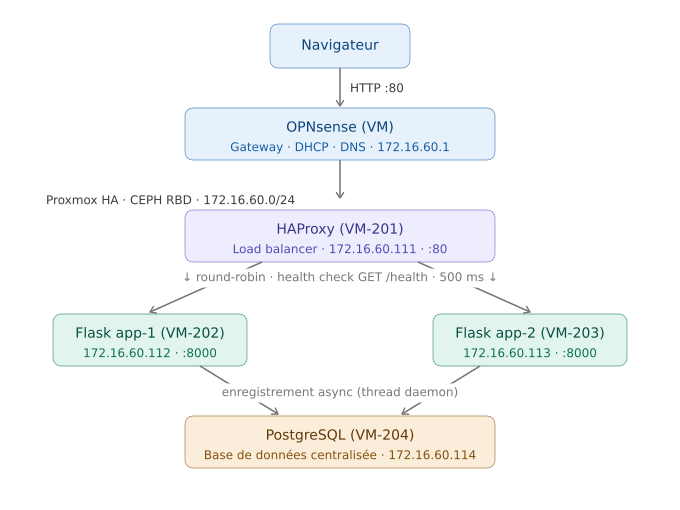
\includegraphics[width=0.85\textwidth]{image/ch3/architecture_sona_web (2).png}
        \caption{Architecture Applicative Sona-Web}
        \label{fig:sona-web}
    \end{center}
\end{figure}

{\color{bleuu} \subsection{Scénario de Validation HA}}

\par Le scénario de démonstration se déroule en quatre temps~: affichage de
l'alternance round-robin entre app-1 et app-2 (validation de l'équilibrage
de charge), puis déclenchement d'une live migration de VM-202 (\texttt{app-1})
vers un autre nœud via la commande \texttt{qm migrate 202 pve-node-2 --online}.

Pendant la migration, Proxmox transfère l'état mémoire de la VM sans arrêter
son exécution~; lorsque la synchronisation atteint \textasciitilde{}99\,\%, la
VM est suspendue quelques dizaines de millisecondes le temps de transférer
le delta final, puis reprend sur le nœud cible. HAProxy détecte l'indisponibilité
transitoire en 200~ms maximum (\texttt{fall 1}) et redirige automatiquement
l'intégralité du trafic vers app-2. Une fois la migration terminée, app-1 est
remise en service dès le premier health check réussi (\texttt{rise 1}).

L'analyse post-migration de la base PostgreSQL confirme qu'aucune requête
n'a été perdue. Le schéma de la table \texttt{requests} comprend les champs
suivants : \texttt{id} (clé primaire), \texttt{instance\_id}, \texttt{path},
\texttt{request\_time} (horodatage automatique), \texttt{client\_ip} et
\texttt{user\_agent}. La requête ci-dessous permet de vérifier la répartition
des requêtes entre les deux instances sur la dernière heure~:

\begin{lstlisting}[language=SQL]
SELECT instance_id,
       COUNT(*) AS total
FROM requests
WHERE request_time > NOW() - INTERVAL '1 hour'
GROUP BY instance_id;
\end{lstlisting}

Ce résultat valide le fonctionnement de la haute disponibilité~: zéro coupure
observable pour l'utilisateur lors d'une migration live sur le cluster Proxmox.

% ============================================================
{\color{bleu} \section{Automatisation}}
% ============================================================

{\color{bleuu} \subsection{Ansible : Périmètre et Playbooks}}

\par Ansible sera utilisé comme outil d'automatisation principal pour trois domaines distincts, chacun correspondant à un playbook dédié.\\

\par \textbf{Playbook 1 : intégration d'un nouveau n\oe{}ud au cluster.} Ce playbook automatisera l'ensemble de la procédure d'intégration d'un serveur fraîchement installé (via PXE) dans le cluster Proxmox existant. Il couvrira la configuration réseau (création des ports VxLAN OVS, assignation des adresses IP sur chaque réseau logique), le peuplement du cluster Corosync, l'initialisation et l'ajout de l'OSD Ceph du nouveau n\oe{}ud, et la configuration des exports de métriques vers InfluxDB.\\

\par \textbf{Playbook 2 : provisionnement de VMs et de conteneurs.} Ce playbook automatisera la création de VMs et de conteneurs LXC à partir de templates cloud-init stockés dans le pool Ceph. Il intégrera la configuration réseau automatique via DHCP (OPNsense dnsmasq), l'assignation au bon bridge OVS (Dev, Prod ou DMZ) selon le paramètre passé, et la configuration initiale du système (mise à jour des paquets, création des comptes Ansible).\\

\par \textbf{Playbook 3 : migration Dev vers Prod ou DMZ.} Ce playbook gérera la promotion d'une VM ou d'un ensemble de VMs de l'environnement de développement vers la production ou la DMZ. Pour les applications microservices, il assurera la reconfiguration réseau de chaque composant, la mise à jour des règles de pare-feu OPNsense correspondantes, et la vérification de la connectivité post-migration.\\

\par Ansible sera exécuté depuis les postes de travail des développeurs via des comptes dédiés sur les n\oe{}uds Proxmox, en utilisant l'accès SSH sur le réseau de management 192.168.10.0/24.\\

{\color{bleuu} \subsection{PXE et TFTP : Provisionnement Automatisé des N\oe{}uds}}

\par Dans une optique de scalabilité horizontale, un pipeline de provisionnement
en deux phases a été mis en place pour automatiser l'intégration de tout nouveau
serveur physique au cluster Proxmox VE, sans aucune intervention manuelle.

\par \textbf{Infrastructure de provisionnement.} Le serveur \textbf{OPNsense}
(adresse \texttt{192.168.10.65}), déjà en charge des services DHCP, DNS et
gateway internet de l'infrastructure, est configuré avec les options DHCP
\texttt{66} (\textit{Next Server}) et \texttt{67} (\textit{Bootfile Name})
pointant vers un conteneur LXC dédié. Ce conteneur héberge le serveur TFTP
ainsi qu'un serveur HTTP Nginx pour la distribution des fichiers d'installation.
Cette architecture évite toute redondance de services DHCP et s'appuie
intégralement sur l'infrastructure réseau existante.

\par \textbf{Phase 1 -- Installation automatique via PXE.} Le protocole
\textbf{PXE} (\textit{Preboot eXecution Environment}) est un standard Intel
gravé dans le firmware des cartes réseau, permettant à une machine de démarrer
depuis le réseau avant toute installation d'un système d'exploitation.
Lorsqu'un nouveau serveur physique est mis sous tension, la séquence suivante
s'exécute automatiquement :

\begin{enumerate}
    \item Le serveur envoie une requête \textbf{DHCP} ; OPNsense lui attribue
    une adresse IP temporaire et lui indique l'adresse du serveur de boot ainsi
    que le fichier bootloader à récupérer ;

    \item Le firmware PXE contacte le serveur \textbf{TFTP}
    (\textit{Trivial File Transfer Protocol}, UDP/69) pour télécharger
    \textit{uniquement} le bootloader (\texttt{pxelinux.0}) et le kernel Linux
    d'amorçage. Le protocole TFTP est retenu à cette étape car il est le seul
    protocole implémentable dans un firmware de quelques dizaines de kilo-octets,
    sans nécessiter de système d'exploitation préalable. Les protocoles FTP, SFTP
    ou SSH sont inutilisables à ce stade, car ils requièrent un OS et des
    bibliothèques logicielles qui n'existent pas encore ;

    \item Une fois le kernel démarré en mémoire vive, l'image d'installation
    Proxmox VE (\textasciitilde{}800 Mo) est téléchargée via \textbf{HTTP} depuis
    le serveur Nginx du conteneur LXC dédié. Ce choix est délibéré : TFTP,
    reposant sur UDP sans mécanisme de reprise sur erreur ni contrôle de flux,
    est inadapté au transfert de fichiers volumineux ; HTTP (TCP) garantit
    l'intégrité et la performance du transfert ;

    \item L'installateur Proxmox lit un fichier de réponses
    (\textit{Answer File} / \texttt{preseed.cfg}), hébergé sur le même serveur
    HTTP, contenant les paramètres d'installation : partitionnement du disque,
    nom d'hôte, fuseau horaire (\texttt{Africa/Algiers}) et langue.
    L'installation s'effectue sans aucune frappe clavier ;

    \item Le serveur redémarre automatiquement sur Proxmox VE
    fraîchement installé.
\end{enumerate}

\par \textbf{Phase 2 -- Intégration au cluster via Ansible.} A l'issue du
redémarrage, le nouveau n\oe{}ud dispose d'un Proxmox VE fonctionnel mais
isolé. Un \textbf{Playbook Ansible} prend alors le relais via SSH pour réaliser
l'intégration complète au cluster existant :

\begin{itemize}
    \item Adhésion au cluster \textbf{Corosync} pour la haute disponibilité ;
    \item Configuration des interfaces \textbf{Open vSwitch} et des tunnels
    \textbf{VxLAN} inter-n\oe{}uds ;
    \item Intégration des disques physiques comme \textbf{OSDs} dans le cluster
    de stockage distribué \textbf{CEPH} ;
    \item Rattachement au groupe \textbf{HA Proxmox}
    (\texttt{sona-ha-group}) ;
    \item Déclaration du n\oe{}ud comme nouvelle cible dans
    \textbf{Prometheus} pour le monitoring existant.
\end{itemize}

\par Ce découpage en deux phases répond à une contrainte technique fondamentale :
PXE et TFTP interviennent dans un environnement \textit{pre-OS} où aucun client
SSH ne peut fonctionner, tandis qu'Ansible nécessite un système d'exploitation
opérationnel et une connectivité SSH, conditions remplies uniquement à l'issue
de la Phase 1. L'ensemble du pipeline permet l'ajout d'un nouveau n\oe{}ud au
cluster en moins de 25 minutes, sans intervention manuelle, répondant ainsi
à l'exigence de scalabilité horizontale du projet.

% ============================================================
{\color{bleu} \section{Architecture du Monitoring}}
% ============================================================

\par La stack de monitoring sera déployée sur une VM dédiée accessible depuis le réseau de management à l'adresse 192.168.10.99. Elle comprendra trois composants complémentaires, chacun couvrant un périmètre de métriques distinct.\\

\par \textbf{Proxmox Metrics Server et InfluxDB.} Proxmox VE supporte nativement l'export de ses métriques générales (CPU, RAM, réseau et stockage des n\oe{}uds et des VMs) vers une base de données InfluxDB via son interface de configuration [15]. Chaque n\oe{}ud poussera automatiquement ses métriques à intervalles réguliers sans nécessiter d'agent supplémentaire. InfluxDB stockera ainsi l'historique complet des métriques d'infrastructure, utilisé à la fois par Grafana pour la visualisation et par le service CLBS pour ses décisions de migration.\\

\par \textbf{Prometheus et Ceph MGR.} Les métriques détaillées du cluster Ceph (état des OSDs, latence des I/O, utilisation du pool, santé du cluster) ne sont pas disponibles via le Proxmox Metrics Server. Le n\oe{}ud MGR actif de Ceph expose nativement un endpoint Prometheus sur le port 9283. Prometheus sera configuré pour scraper cet endpoint, fournissant ainsi une visibilité complète sur la santé du stockage distribué.\\

\par \textbf{Grafana.} Grafana sera connecté à la fois à InfluxDB et à Prometheus comme sources de données, permettant de construire des tableaux de bord unifiés couvrant l'ensemble de l'infrastructure : utilisation des ressources par n\oe{}ud, état du cluster Ceph, historique des migrations CLBS, et alertes de surcharge.\\


% %%%%%%%%%%%%%%%%%%%%%%%%%%%%%%%%%%%%%%%%%%%%%%%%%%%%%%%%%%%%
% PARTIE 2 : STORAGE
% %%%%%%%%%%%%%%%%%%%%%%%%%%%%%%%%%%%%%%%%%%%%%%%%%%%%%%%%%%%%

{\color{bleu} \section{Partie II : Storage}}

% ============================================================
{\color{bleu} \section{Architecture du Stockage Ceph}}
% ============================================================

{\color{bleuu} \subsection{Composants du Cluster Ceph}}

\par Le cluster Ceph sera composé des services suivants, répartis sur les trois n\oe{}uds physiques :

\begin{itemize}
    \item \textbf{Monitors (MON) :} un monitor par n\oe{}ud, soit trois au total. Les monitors maintiennent la carte du cluster (cluster map) et assurent le consensus distribué. Trois monitors garantissent un quorum stable (2/3 suffisants).
    \item \textbf{Managers (MGR) :} le n\oe{}ud PVE-02 hébergera le MGR actif, PVE-03 le MGR en standby. Le MGR expose les métriques du cluster via une interface REST utilisée par notre stack de monitoring Prometheus.
    \item \textbf{OSDs (Object Storage Daemons) :} un OSD par n\oe{}ud sur le disque sdb (300 GB SAS), soit trois OSDs au total contribuant au pool de stockage distribué.
\end{itemize}

{\color{bleuu} \subsection{Dimensionnement du Pool}}

\par Avec un facteur de réplication de 3, la capacité utilisable est :\\
\par \textbf{Capacité utilisable = (3 x 300 GB) / 3 = 300 GB}\\

\par L'algorithme CRUSH sera configuré pour respecter les domaines de défaillance au niveau du n\oe{}ud physique, garantissant que les trois répliques d'un même bloc ne se retrouveront jamais sur le même serveur physique [12]. Le tableau suivant présente la répartition prévue du stockage :\\

\begin{center}
\begin{tabular}{|p{7cm}|p{5cm}|}
\hline
\textbf{Usage} & \textbf{Stockage alloué} \\
\hline
VM OPNsense & 20 GB \\
\hline
HAProxy VM & 16 GB \\
\hline
Apache VM 1 & 32 GB \\
\hline
Apache VM 2 & 32 GB \\
\hline
PostgreSQL VM & 100 GB \\
\hline
VM Monitoring (InfluxDB + Prometheus + Grafana) & 100 GB \\
\hline
VM CLBS & 32 GB \\
\hline
Marge, snapshots et templates & \textasciitilde{}200 GB \\
\hline
\textbf{Total estimé} & \textbf{\textasciitilde{}532 GB (thin provisioning)} \\
\hline
\end{tabular}
\end{center}
\noindent \textit{Tableau 3-4 : Répartition du stockage Ceph par usage}\\

\par Le total estimé dépasse la capacité brute de 300 GB car le thin provisioning de Ceph RBD ne consomme l'espace que proportionnellement aux données réellement écrites, les volumes étant alloués à la création mais non pré-remplis.\\

{\color{bleuu} \subsection{Configuration CRUSH et Domaines de Défaillance}}

\par Lors de la création du cluster Ceph via Proxmox VE, une règle
CRUSH par défaut est générée automatiquement, organisant les OSDs
selon la hiérarchie \texttt{root > host > osd} avec la politique
\texttt{chooseleaf firstn 0 type host}. Cela garantit que les trois
répliques d'un même objet sont placées sur trois hôtes physiques
distincts, sans aucune configuration manuelle. Un point mérite
attention : avec \texttt{size=3} et seulement 3 OSDs sur 3 hôtes,
la perte d'un n\oe{}ud place le pool en état \texttt{degraded}.
Le paramètre \texttt{min\_size=2} (valeur par défaut Ceph) maintient
le pool accessible en lecture et écriture dans cet état ; il convient
de vérifier qu'il n'a pas été modifié lors de la création du pool.\\

\begin{center}
\begin{tabular}{|p{4cm}|p{9cm}|}
\hline
\textbf{Paramètre} & \textbf{Valeur et origine} \\
\hline
Domaine de défaillance & \texttt{host} -- généré automatiquement par Proxmox \\
\hline
Facteur de réplication (\texttt{size}) & 3 -- une réplique par n\oe{}ud physique \\
\hline
\texttt{min\_size} & 2 (défaut Ceph) -- pool accessible avec 2 n\oe{}uds opérationnels \\
\hline
\end{tabular}
\end{center}
\noindent \textit{Tableau 3-X : Paramètres CRUSH appliqués automatiquement par Proxmox}\\


% %%%%%%%%%%%%%%%%%%%%%%%%%%%%%%%%%%%%%%%%%%%%%%%%%%%%%%%%%%%%
% PARTIE 3 : NETWORK
% %%%%%%%%%%%%%%%%%%%%%%%%%%%%%%%%%%%%%%%%%%%%%%%%%%%%%%%%%%%%

{\color{bleu} \section{Partie III : Network}}

% ============================================================
{\color{bleu} \section{Architecture Réseau}}
% ============================================================

{\color{bleuu} \subsection{Contexte et Contraintes Réseau}}

\par Le réseau de Sonatrach met à disposition un sous-réseau 192.168.10.0/24 déjà opérationnel, correspondant au réseau de management. Ce réseau est utilisé pour l'accès SSH aux n\oe{}uds Proxmox depuis les postes de travail ainsi que pour l'interface web d'administration Proxmox. La connectivité Internet des n\oe{}uds est assurée par un poste de travail jouant le rôle de routeur externe, configuré à l'adresse 192.168.10.36, qui réalise du NAT et du forwarding IP pour donner aux serveurs un accès réseau sortant.\\

\par Le switch de Sonatrach autorise uniquement le VLAN 10 natif et n'autorise pas la configuration de VLANs supplémentaires pour des raisons de sécurité interne. Afin de créer les réseaux logiques supplémentaires nécessaires à l'infrastructure, nous retenons \textbf{VxLAN (Virtual Extensible LAN)} comme technologie d'encapsulation. VxLAN permet de créer des réseaux logiques de niveau 2 tunnelisés au-dessus du réseau IP existant (192.168.10.0/24), sans nécessiter aucune modification de la configuration du switch. Open vSwitch gérera la création et la terminaison de ces tunnels sur chaque n\oe{}ud Proxmox. Cette approche est transparente pour Proxmox et pour Ceph, qui voient des interfaces réseau standards sans avoir conscience du mécanisme d'encapsulation sous-jacent.\\

{\color{bleuu} \subsection{Topologie Réseau Retenue}}

\par La topologie réseau retenue s'articule autour de deux niveaux de segmentation complémentaires, illustrée en figure 3-2.\\

\par \textbf{Niveau 1 : réseaux d'infrastructure (VxLAN inter-n\oe{}uds).} Pour les réseaux de contrôle de la plateforme (Corosync, Ceph Cluster, Ceph Public, Live Migration), des tunnels VxLAN point-à-point en maillage complet seront établis entre les trois n\oe{}uds via Open vSwitch. Chaque n\oe{}ud créera deux ports VxLAN vers chacun des deux autres n\oe{}uds, garantissant une connectivité directe sans point de transit central.\\

\par \textbf{Niveau 2 : réseaux internes des VMs (OPNsense).} Pour les réseaux applicatifs (Dev, Prod, DMZ), nous retenons une architecture centralisée autour d'une VM OPNsense dédiée. Trois bridges OVS internes seront configurés sur chaque n\oe{}ud Proxmox (un par réseau applicatif). La VM OPNsense disposera de quatre interfaces réseau virtuelles : une interface WAN connectée au réseau de management (192.168.10.65, avec passerelle vers le routeur externe 192.168.10.36), et trois interfaces LAN connectées respectivement aux bridges Dev, Prod et DMZ. OPNsense assurera le routage inter-réseaux, le NAT vers Internet, et les règles de pare-feu applicatives.\\

\par Afin de permettre aux n\oe{}uds Proxmox d'accéder directement aux VMs internes (172.16.x.0/24) sans passer par le routeur externe, une route statique sera configurée sur le poste de travail routeur (192.168.10.36) pour rediriger tout trafic à destination des sous-réseaux 172.16.0.0/16 vers l'adresse WAN d'OPNsense (192.168.10.65). Cette approche évite tout hairpin NAT et conserve une architecture claire.\\

\begin{figure}[H]
    \begin{center}
        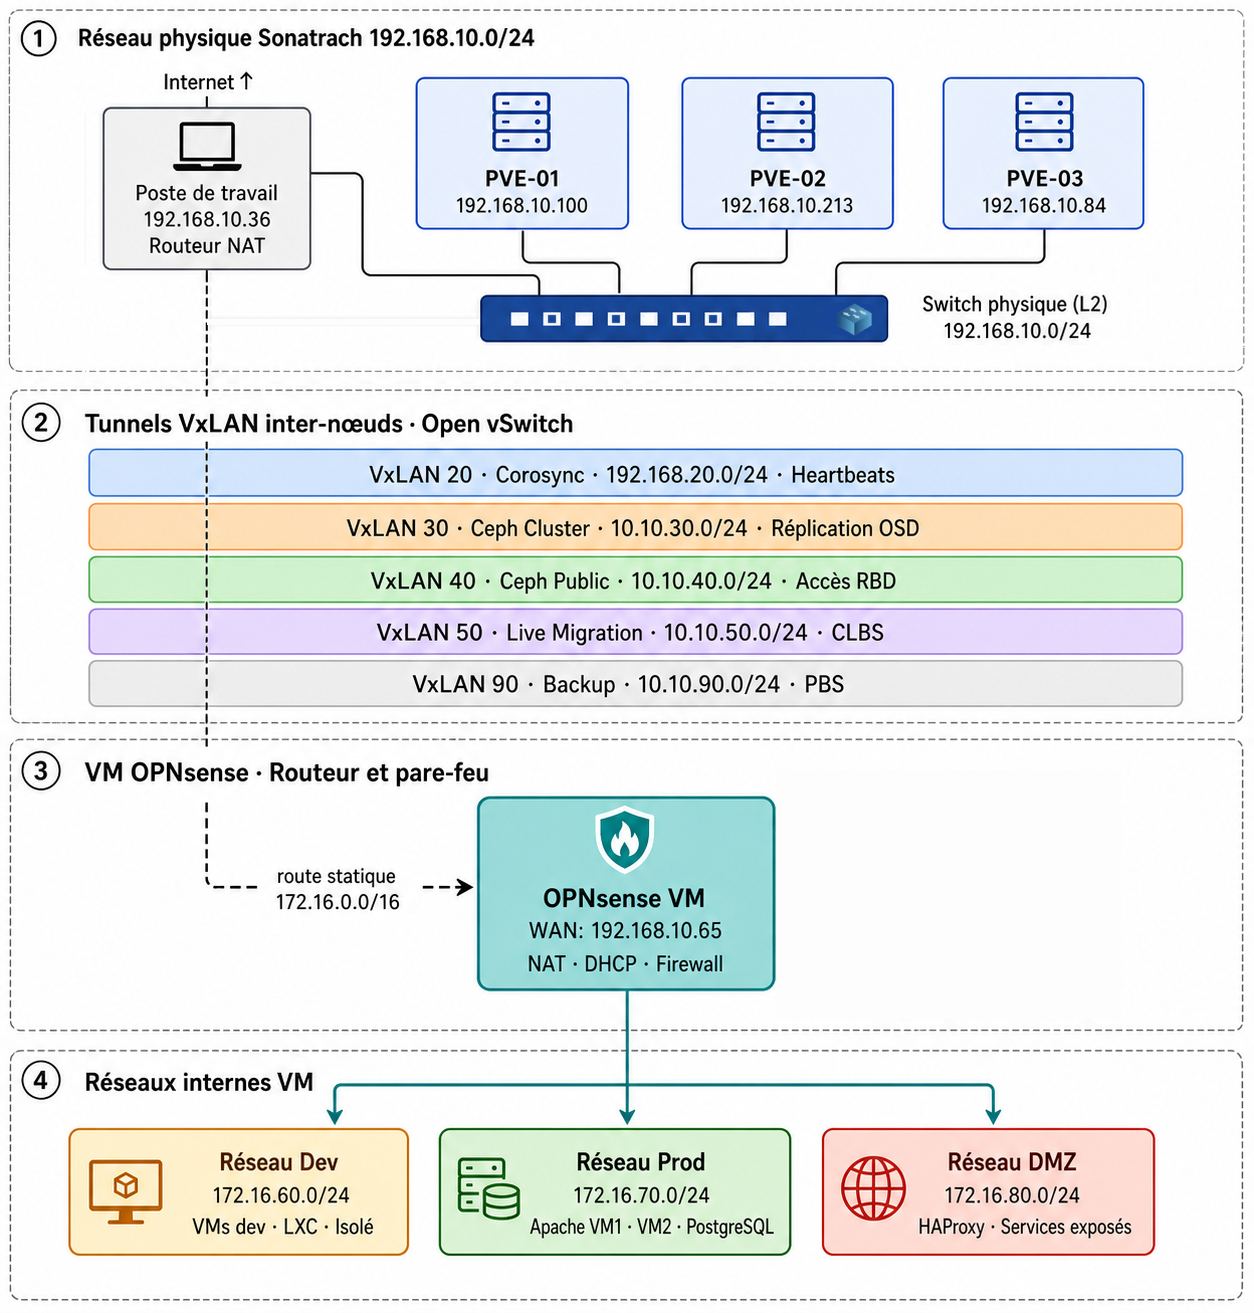
\includegraphics[width=0.9\textwidth]{image/ch3/architecture reseau.png}
        \caption{Topologie Réseau et Plan VxLAN}
        \label{fig:topologie-reseau}
    \end{center}
\end{figure}

{\color{bleuu} \subsection{Bridges Open vSwitch par N\oe{}ud}}

\par Chaque n\oe{}ud Proxmox expose quatre bridges Open vSwitch identiques, constituant les points d'attachement réseau pour toutes les VMs et les tunnels VxLAN. Le tableau suivant décrit leur rôle et leur configuration :\\

\begin{center}
\begin{tabular}{|p{2.5cm}|p{3cm}|p{3cm}|p{5cm}|}
\hline
\textbf{Bridge OVS} & \textbf{VxLAN associé} & \textbf{Sous-réseau} & \textbf{Rôle} \\
\hline
\texttt{vmbr0} & réseau physique natif & 192.168.10.0/24 & Bridge principal. Accès management, SSH, Web UI Proxmox, monitoring, interface WAN d'OPNsense.\\
\hline
\texttt{vmbr60} & \texttt{vxlan60-int} & 172.16.60.0/24 & Réseau Dev. OPNsense y expose son interface LAN1. \\
\hline
\texttt{vmbr70} & \texttt{vxlan70-int} & 172.16.70.0/24 & Réseau Prod. OPNsense y expose son interface LAN2. \\
\hline
\texttt{vmbr80} & \texttt{vxlan80-int} & 172.16.80.0/24 & Réseau DMZ. OPNsense y expose son interface LAN3. \\
\hline
\end{tabular}
\end{center}
\noindent \textit{Tableau 3-X : Bridges OVS et tunnels VxLAN par n\oe{}ud Proxmox}\\

\par Les interfaces \texttt{vxlan60-int}, \texttt{vxlan70-int} et \texttt{vxlan80-int} sont des ports VxLAN OVS point-à-multipoint établis entre les trois n\oe{}uds, permettant à une VM connectée à \texttt{vmbr60} sur PVE-01 de communiquer de manière transparente avec une VM connectée au même bridge sur PVE-02 ou PVE-03, sans aucune configuration supplémentaire au niveau de la VM.\\

{\color{bleuu} \subsection{Plan d'Adressage}}

\par Le plan d'adressage est organisé en deux familles de réseaux. Les réseaux VxLAN d'infrastructure interconnectent les n\oe{}uds Proxmox entre eux pour les flux de contrôle et de données de la plateforme. Les réseaux applicatifs internes sont gérés par OPNsense et hébergent les VMs et conteneurs.\\

\par \textbf{Réseaux VxLAN d'infrastructure :}
\begin{itemize}
    \item \textbf{VxLAN 10 -- Management (192.168.10.0/24, passerelle 192.168.10.36) :} Web UI Proxmox, SSH, API (réseau physique existant).
    \item \textbf{VxLAN 20 -- Corosync (192.168.20.0/24) :} Heartbeats et quorum cluster.
    \item \textbf{VxLAN 30 -- Ceph Cluster (10.10.30.0/24) :} Réplication OSD interne.
    \item \textbf{VxLAN 40 -- Ceph Public (10.10.40.0/24) :} Accès VMs au stockage RBD.
    \item \textbf{VxLAN 50 -- Live Migration (10.10.50.0/24) :} Migrations à chaud et CLBS.
\end{itemize}

\par \textbf{Réseaux applicatifs internes (gérés par OPNsense) :}
\begin{itemize}
    \item \textbf{Réseau Dev (172.16.60.0/24, passerelle OPNsense LAN1 172.16.60.1) :} environnements de développement et de test.
    \item \textbf{Réseau Prod (172.16.70.0/24, passerelle OPNsense LAN2 172.16.70.1) :} environnements de production.
    \item \textbf{Réseau DMZ (172.16.80.0/24, passerelle OPNsense LAN3 172.16.80.1) :} services exposés, dont HAProxy.
\end{itemize}

\begin{center}
\begin{tabular}{|p{1.8cm}|p{2.8cm}|p{2.5cm}|p{2.5cm}|p{2.5cm}|p{2.5cm}|}
\hline
\textbf{N\oe{}ud} & \textbf{Management} & \textbf{VxLAN 20 Corosync} & \textbf{VxLAN 30 Ceph Cluster} & \textbf{VxLAN 40 Ceph Public} & \textbf{VxLAN 50 Migration} \\
\hline
PVE-01 & 192.168.10.100 & 192.168.20.11 & 10.10.30.11 & 10.10.40.11 & 10.10.50.11 \\
\hline
PVE-02 & 192.168.10.213 & 192.168.20.12 & 10.10.30.12 & 10.10.40.12 & 10.10.50.12 \\
\hline
PVE-03 & 192.168.10.84  & 192.168.20.13 & 10.10.30.13 & 10.10.40.13 & 10.10.50.13 \\
\hline
\end{tabular}
\end{center}
\noindent \textit{Tableau 3-3 : Adressage IP statique des n\oe{}uds Proxmox par réseau logique}\\

{\color{bleuu} \subsection{VM OPNsense : Routeur et Pare-feu Centralisé}}

\par La VM OPNsense constituera le coeur du réseau applicatif. Il s'agit d'une distribution FreeBSD dédiée aux fonctions de routage et de sécurité réseau, reconnue pour sa richesse fonctionnelle et sa robustesse en environnement virtualisé. Dans notre architecture, OPNsense sera déployée avec quatre interfaces réseau virtuelles :

\begin{itemize}
    \item \textbf{Interface WAN (192.168.10.65/24) :} connectée au bridge OVS du réseau de management, avec la passerelle 192.168.10.36 (routeur externe). Cette interface assure l'accès Internet sortant via NAT pour toutes les VMs internes.
    \item \textbf{Interface LAN1 (172.16.60.1/24) :} passerelle du réseau Dev.
    \item \textbf{Interface LAN2 (172.16.70.1/24) :} passerelle du réseau Prod.
    \item \textbf{Interface LAN3 (172.16.80.1/24) :} passerelle du réseau DMZ.
\end{itemize}

\par OPNsense intègre nativement dnsmasq, que nous utiliserons comme serveur DHCP pour les trois réseaux internes. L'attribution d'adresses IP aux VMs et conteneurs sera ainsi automatisée dès leur connexion à l'un des bridges applicatifs, ce qui simplifiera le provisionnement dans les playbooks Ansible.\\

{\color{bleuu} \subsection{Haute Disponibilité d'OPNsense}}

\par OPNsense étant le point central du routage inter-réseaux et du
filtrage applicatif, sa défaillance isolerait l'ensemble des réseaux
internes. Dans notre architecture, la résilience d'OPNsense est
assurée par son intégration au groupe HA Proxmox (\texttt{sona-ha-group}).\\

\par En cas de défaillance du n\oe{}ud hébergeant la VM OPNsense,
Corosync détecte la panne et le HA Manager de Proxmox déclenche
automatiquement le redémarrage de la VM sur l'un des deux n\oe{}uds
survivants. La VM redémarre directement depuis son volume Ceph RBD,
sans transfert de données préalable, ce qui minimise le temps de
reprise. Ce délai de basculement est typiquement compris entre 60 et
120 secondes, pendant lesquels le trafic inter-réseaux est interrompu.\\

\par Cette approche offre une reprise automatique après panne sans
nécessiter de déploiement d'une seconde instance OPNsense. Elle
constitue un compromis adapté au contexte de notre infrastructure de
démonstration : le RTO de 60 à 120 secondes est acceptable pour les
scénarios de validation visés. Une architecture de production
nécessitant un basculement transparent pourrait évoluer vers une
configuration active/passive avec le protocole CARP, natif dans
OPNsense, qui réduirait ce délai à moins de 5 secondes.\\

% ============================================================
{\color{bleu} \section{Architecture du Pare-feu}}
% ============================================================

\par La conception du pare-feu s'articule sur deux niveaux complémentaires : le pare-feu applicatif centralisé dans OPNsense, et le pare-feu d'hyperviseur natif de Proxmox VE. Cette complémentarité est illustrée en figure 3-3.\\

{\color{bleuu} \subsection{Pare-feu OPNsense : Filtrage Inter-réseaux}}

\par OPNsense appliquera les politiques de filtrage entre les réseaux applicatifs Dev, Prod et DMZ, ainsi que les règles d'accès Internet. Les règles retenues pour notre conception sont les suivantes :\\

\textbf{Règles autorisées :}
\begin{itemize}
    \item Dev vers WAN (Internet) : autorisé pour les mises à jour et les dépôts de paquets.
    \item DMZ vers WAN (Internet) : autorisé pour les services exposés nécessitant un accès sortant.
    \item Prod vers DMZ : autorisé afin de permettre aux services de production de communiquer avec les composants exposés (HAProxy, etc.).
\end{itemize}

\textbf{Règles bloquées :}
\begin{itemize}
    \item Dev vers Prod : bloqué. Les environnements de développement ne doivent pas avoir accès direct aux ressources de production.
    \item Dev vers DMZ : bloqué. Les services de développement ne doivent pas être accessibles ou accéder aux services exposés publiquement.
    \item Prod vers WAN direct : bloqué. Le trafic de production à destination d'Internet passera obligatoirement par la DMZ.
\end{itemize}

{\color{bleuu} \subsection{Pare-feu Proxmox : Filtrage au Niveau Hyperviseur}}

\par Proxmox VE intègre nativement un mécanisme de pare-feu basé sur iptables, configurable à trois niveaux : cluster, n\oe{}ud et VM individuelle [6]. Nous exploiterons ce mécanisme pour une couche de protection complémentaire au niveau de l'hyperviseur, indépendante d'OPNsense.\\

\par Au niveau du cluster, nous définirons un ensemble de règles globales visant à protéger les interfaces de management et à isoler les réseaux d'infrastructure. Les règles de conception retenues sont les suivantes :

\begin{itemize}
    \item \textbf{Isolation des réseaux Ceph :} interdire tout trafic provenant des réseaux applicatifs (172.16.x.0/24) à destination des réseaux Ceph Cluster (VxLAN 30) et Ceph Public (VxLAN 40). Ces réseaux sont réservés à l'usage exclusif des n\oe{}uds Proxmox.
    \item \textbf{Isolation du réseau Corosync :} interdire tout accès extérieur au réseau VxLAN 20. Seuls les n\oe{}uds Proxmox communiqueront sur ce réseau.
    \item \textbf{Protection de l'interface de management :} restreindre l'accès à l'interface web Proxmox (port 8006) et SSH (port 22) aux seules adresses du sous-réseau 192.168.10.0/24.
    \item \textbf{Limitation des accès inter-VMs :} au niveau de chaque VM, n'autoriser que les ports applicatifs nécessaires, en suivant le principe du moindre privilège.
\end{itemize}

\begin{figure}[H]
    \begin{center}
        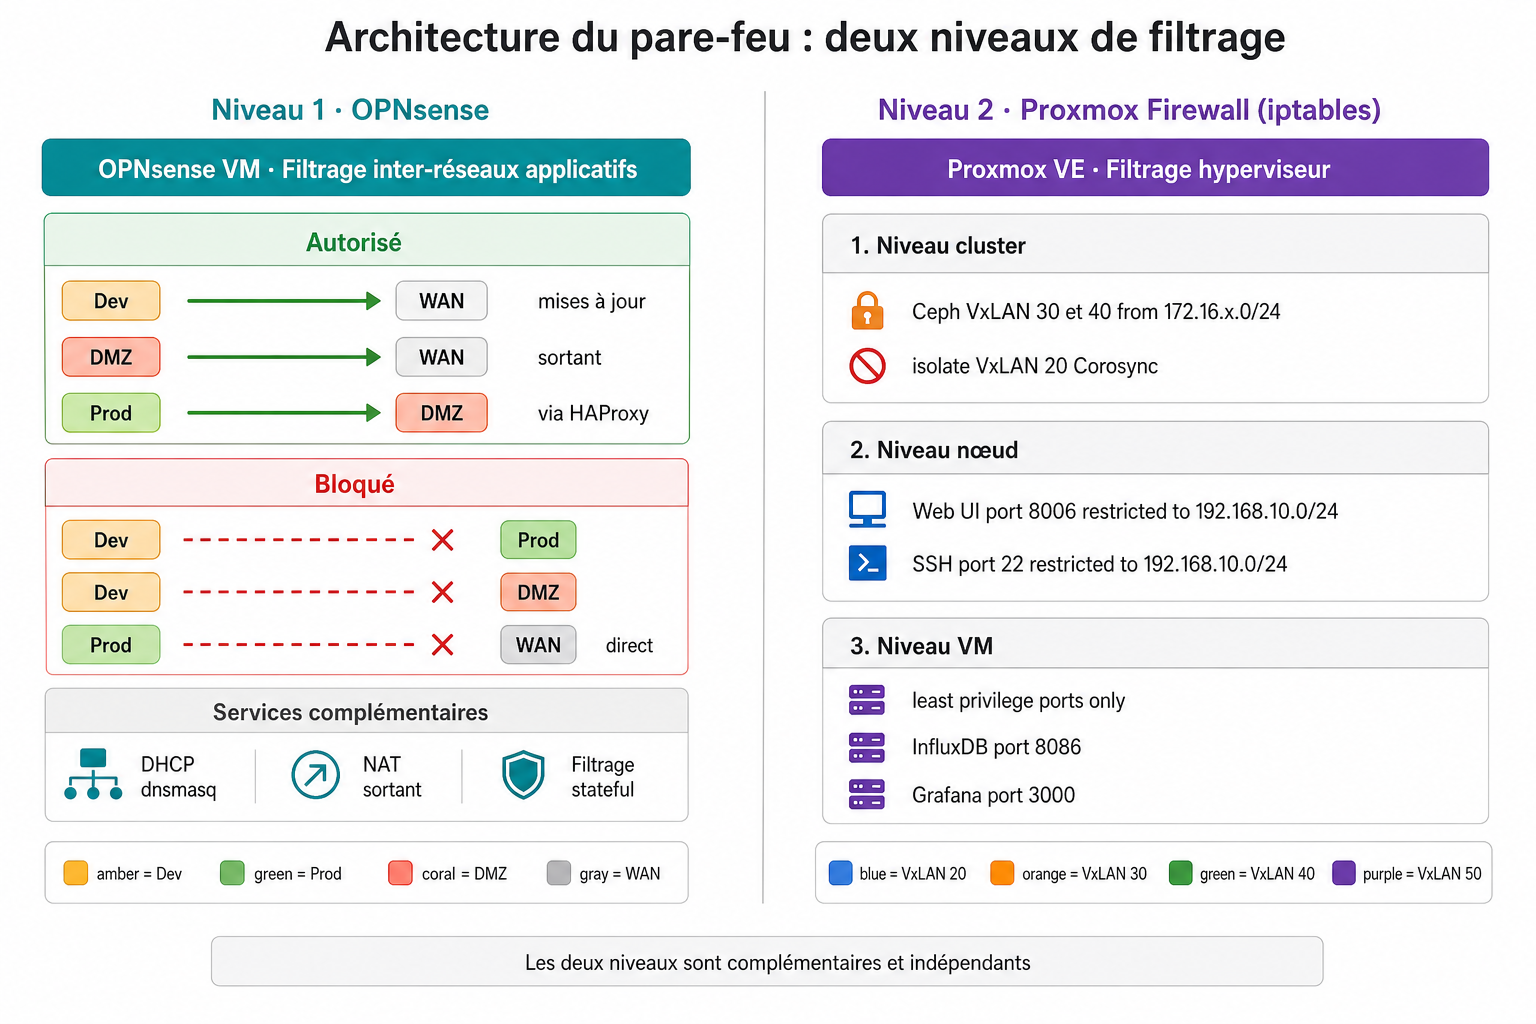
\includegraphics[width=0.9\textwidth]{image/ch3/firewall.png}
        \caption{Architecture du Pare-feu : OPNsense et Proxmox Firewall}
        \label{fig:firewall}
    \end{center}
\end{figure}


% %%%%%%%%%%%%%%%%%%%%%%%%%%%%%%%%%%%%%%%%%%%%%%%%%%%%%%%%%%%%
% CONCLUSION
% %%%%%%%%%%%%%%%%%%%%%%%%%%%%%%%%%%%%%%%%%%%%%%%%%%%%%%%%%%%%

% ============================================================
{\color{bleu} \section{Conclusion}}
% ============================================================

\par Ce chapitre a présenté la conception complète de l'infrastructure Cloud privée hyperconvergée proposée, organisée autour des trois piliers fondamentaux de l'HCI. La partie Compute couvre les trois n\oe{}uds physiques Proxmox bare metal sur serveurs Dell PowerEdge R720, le cluster Proxmox avec son mécanisme de quorum Corosync et de haute disponibilité, le mécanisme d'équilibrage proactif CLBS adapté du CSLB, l'application de démonstration Sona-Web, ainsi que l'automatisation via Ansible et PXE. La partie Storage détaille le cluster Ceph avec ses composants MON/MGR/OSD, le dimensionnement du pool et la politique de thin provisioning. La partie Network expose l'architecture VxLAN inter-noeuds gérée par Open vSwitch, le plan d'adressage complet, le routage centralisé via OPNsense, et le plan de pare-feu à deux niveaux. L'ensemble de ces choix de conception constitue une base cohérente et documentée pour la phase d'implémentation présentée dans le chapitre suivant.\\